%%%%%%%%%%%%%%%%%%%%%%%%%%%%%%%%%%%%%%%%%%%%%%%%%%%%%%%%%%%%%%%%%%%%%%%%%%%%%%%%
%2345678901234567890123456789012345678901234567890123456789012345678901234567890
%        1         2         3         4         5         6         7         8

\documentclass[letterpaper, 10 pt, conference]{ieeeconf}  % Comment this line out if you need a4paper

%\documentclass[a4paper, 10pt, conference]{ieeeconf}      % Use this line for a4 paper

\IEEEoverridecommandlockouts                              % This command is only needed if 
                                                          % you want to use the \thanks command

\overrideIEEEmargins                                      % Needed to meet printer requirements.

\usepackage{lmodern}
\usepackage{textcomp}
\usepackage{amsmath}
\usepackage{lipsum}
\usepackage{hyperref}

\usepackage{graphicx}
\graphicspath{ {img/} }

\newcommand{\norm}[1]{\left\lVert#1\right\rVert}


\title{
Topic Proposal: \\Interaction between task and motion planning
}


\author{
Gudjon Einar Magnusson
\\ \href{mailto:gmagnusson@fc-md.umd.edu}{\tt\small gmagnusson@fc-md.umd.edu}
}


\begin{document}


\maketitle
\thispagestyle{empty}
\pagestyle{empty}


%%%%%%%%%%%%%%%%%%%%%%%%%%%%%%%%%%%%%%%%%%%%%%%%%%%%%%%%%%%%%%%%%%%%%%%%%%%%%%%%
\begin{abstract}

Task planners tend to have an overly simplified view of the world. Motion planners are short sighted and fail to see the big picture. I propose to implement a planner that integrates task and motion planning to produce better plans in a semi structured environment. 

\end{abstract}


%%%%%%%%%%%%%%%%%%%%%%%%%%%%%%%%%%%%%%%%%%%%%%%%%%%%%%%%%%%%%%%%%%%%%%%%%%%%%%%%
\section{Introduction}

Task planning and motion planning are both mature fields that offer a verity of advanced algorithms to solve their respective problems. However, when we try to implements robots to carry out increasingly complex tasks it becomes clear that there is much room for improvement in the interaction between these two domains. 

Task planners can find a long sequence of actions to carry out a task under complex logical constraints. These planner abstract away the properties of the physical world they operate in, they fail to consider how actions may affect the robots configuration space.

Motion planners can find a optimal or near optimal path to move a physical object through space while avoiding collisions and respecting dynamic constraints. They generally operate over the time scale of a single task and fail to consider how the current motion may interferer with future tasks.

Currently, in production environments these problems are avoided by structuring the robots environments such that the robots motion and geometry does not interferer with task planning and the simplified assumptions made by the task planner generally hold. That way you can get away with using the task planner to get a sequence of actions and calling the motion planner once per task to carry it out, and not worry about any interference between the two. However, if we want future robots to be able to carry out sophisticated tasks in unstructured or semi-structured environments, we need to develop methods that are more cognizant during that during the planning and execution of actions.


\label{fig}
\section{Related Work}

A verity of methods have been proposed to tackle some aspect of this problem, but there are no obvious solutions that can be directly applied. 
\cite{hpn2} describes a robot that moves a number of object around a confined space while making sure those objects stay out of the sweep area of future actions. \cite{waipointSequence} describes how a motion planner can use knowledge of the task plan to optimize the path chosen for the current task so the motion forms a more continuous sequence. \cite{asymov} describes a planner that bridges the gap between symbolic and geometric reasoning so that the task planner can deal with geometric preconditions and effects of actions. \cite{ffrob} proposes a heuristic method for efficient forward search task planning while taking geometric and kinematic constraints into account.

Based on my preliminary research it seams that aSyMov\cite{asymov}\cite{asymov2} is the most mature implementation that directly deals with this specific problem. 


\section{Personal Motivation}

I picked this project because I am passioned about cognitive robotics. My background is in computer science and AI but in that field the physical world tends to be abstracted away, and motion planning is oversimplified to an 8-connected grid. My hope is that this project will extend my understanding of AI planning to include the complexity of infinite state spaces and dynamic constraints. 


\section{Intended methodology}

\subsection{Vehicle Description}

To guide and demonstrate my research I intend to implement my planner for an autonomous fork-lift that is intended to operate in a semi-structured environment. By semi-structured I mean that the robot has a map if the floor layout but does not have perfect knowledge of all objects in the environment. Possible driving paths are not predefined but must be solved on the fly. Any driving path that does not cause a collision with the robot or its cargo is considered valid.

\begin{figure}[h]
\centering
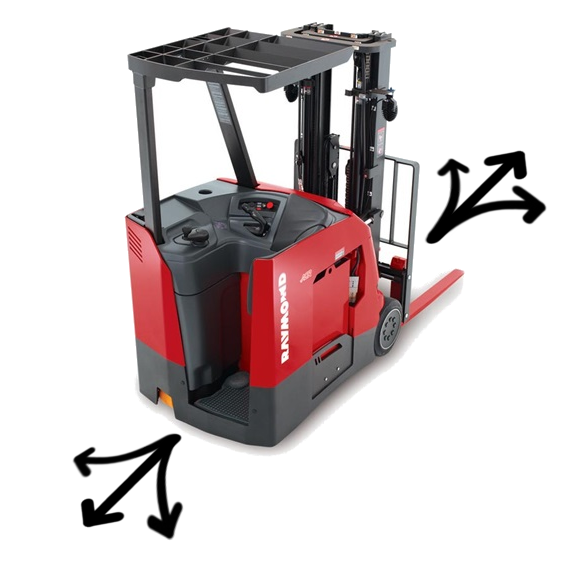
\includegraphics[width=0.25\textwidth]{forklift}
\caption{My implementation will control a forklift similar to this one}
\label{fig:forklift}
\end{figure}

The robot controls are similar that of a car. It can drive forward and backward and can turn right and left with a limited but variable turning radius (it can not turn on the spot). This puts some constraints on how it can navigate the environment. The robot can pick up cargo with the forks on the front of the vehicle. In order to pick up cargo the robot must first align with it so the forks are in the right place. Cargo can be placed anywhere, as long as its not in collision. 


\subsection{Software Packages}

I plan to operate my forklift in simulation using ROS and Gazebo. ROS conveniently allows me to skip much of the boilerplate required to get a robot up and running in simulation, so I can go straight to implementing the task and motion planner. 

I expect to base much of my implementation on the aSyMov planner but will investigate every opportunity I see to add improvements. Most of the code will be written in python because it allows for very rapid development and is well supported by ROS.


\section{Conclusion}

I have laid out an ambitious plan to implement an intelligent, autonomous fork-lift, operating in a complicated environment. My plan is demonstrate all of the concepts I explained above, but I  recognize that every plan is likely to change on its first encounter with implementation. Luckily I think that the fork-lift scenario I described is very flexible and could easily be extended or simplified.

To conclude I want to boil down my main metric of success for of this project. At the end of this project I want to demonstrate a robot that can efficiently plan and execute a long sequence of tasks without the need to explicitly enumerate the possible states of objects and actors in the system.



\addtolength{\textheight}{-12cm}   % This command serves to balance the column lengths
                                  % on the last page of the document manually. It shortens
                                  % the textheight of the last page by a suitable amount.
                                  % This command does not take effect until the next page
                                  % so it should come on the page before the last. Make
                                  % sure that you do not shorten the textheight too much.

%%%%%%%%%%%%%%%%%%%%%%%%%%%%%%%%%%%%%%%%%%%%%%%%%%%%%%%%%%%%%%%%%%%%%%%%%%%%%%%%


\bibliography{ref}
\bibliographystyle{ieeetr}

\end{document}
